\section{Geometria}

\questao{(OM$^3$SP 2026 - 1ª Fase) O professor Genílson estava fazendo uma obra em casa e usou sua grande escada para auxiliar na pintura superior de sua parede. Sabe-se que a distância da base da escada até a parede mede $12 m$. Ele também sabe que a escada tem $13m$ de comprimento. A que altura esta escada se encontra do chão?}
        \begin{multicols}{4}
            \begin{enumerate}[label=\alph*)]
                \item $4m$
                \item $5m$
                \item $6m$
                \item $7m$
        \end{enumerate}
        \end{multicols}

\begin{solucoes}{1}
    \solucao
    No problema do professor Genilson se tem a situação a seguir,
        \begin{figure}[H]
            \centering
            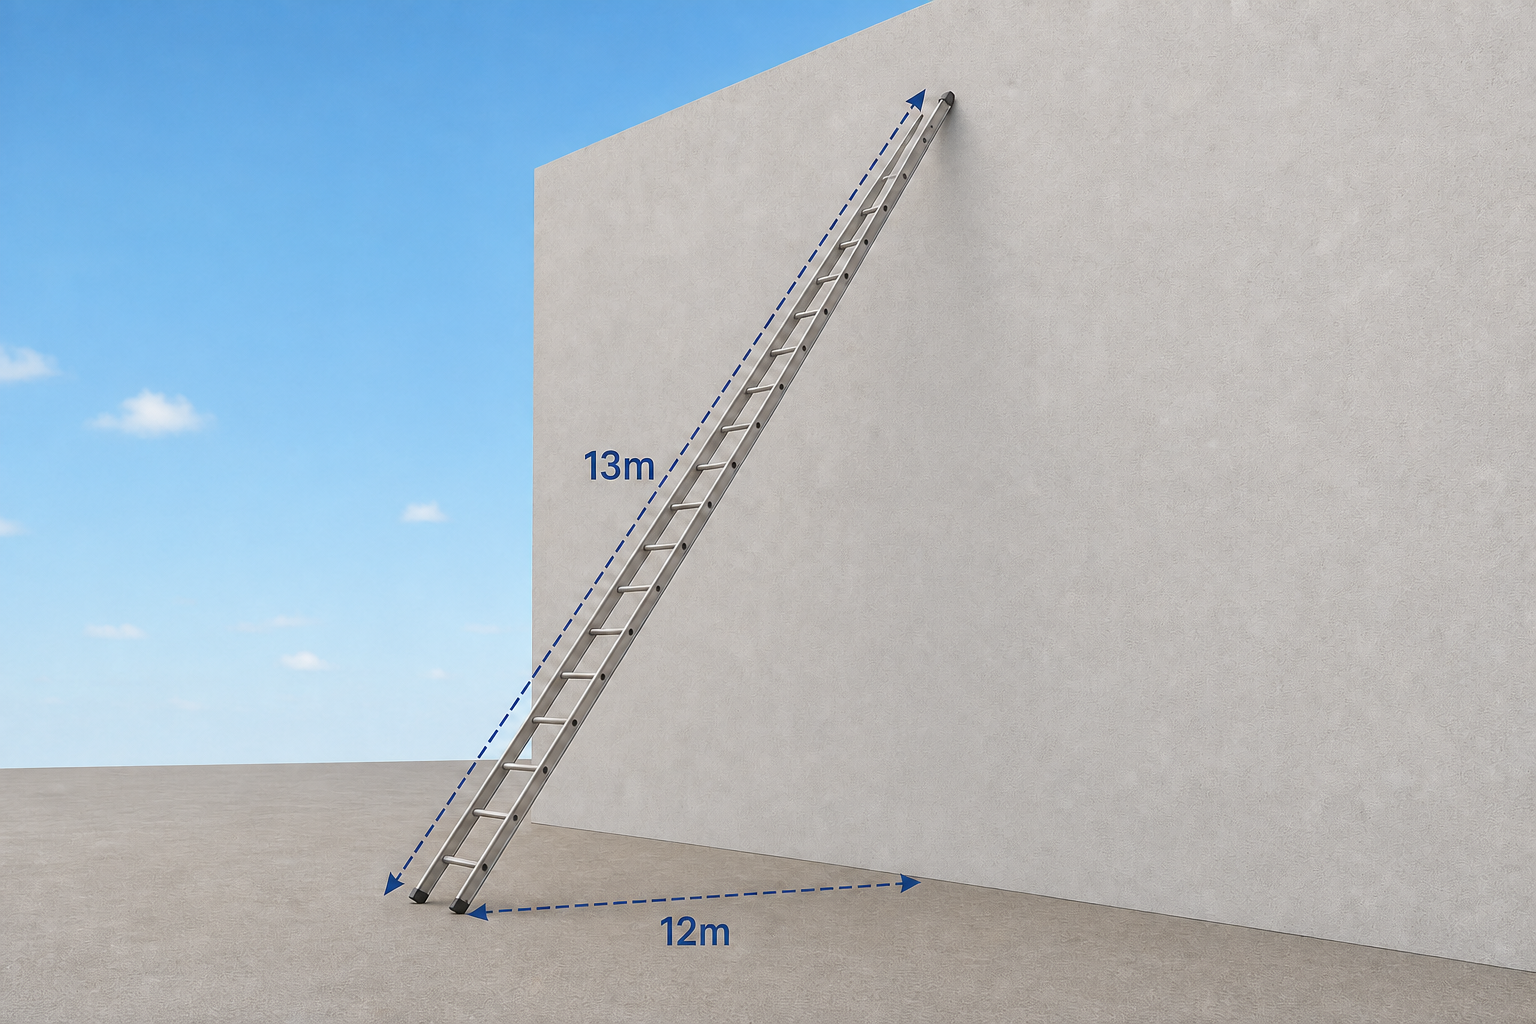
\includegraphics[width=0.5\linewidth]{figuras/9_ano/IMG_0937.png}
        \end{figure}
        Como o triângulo gerado é retângulo, pode-se utilizar o teorema de Pitágoras. Com isso, 
        \begin{equation*}
            13^2=12^2+x^2
        \end{equation*}
        \begin{equation*}
            169=144+x^2
        \end{equation*}
        \begin{equation*}
           x^2=169-144
        \end{equation*}
        \begin{equation*}
         x^2=25
        \end{equation*}
        \begin{equation*}
            x=\sqrt{25}=5
        \end{equation*}
        Sendo assim, a altura da escada até o chão é de $5m$.\\
        \textbf{ALTERNATIVA B}
\end{solucoes}

\questao{(OM$^3$SP 2026 - 1ª Fase) A professora Elielma acabou de comprar uma mansão e na sala de estar de sua mansão, existe uma escada em formato de caracol (espiral) ligando o andar térreo ao andar superior, conforme mostra à imagem a seguir:}
          \begin{figure}[H]
            \centering
            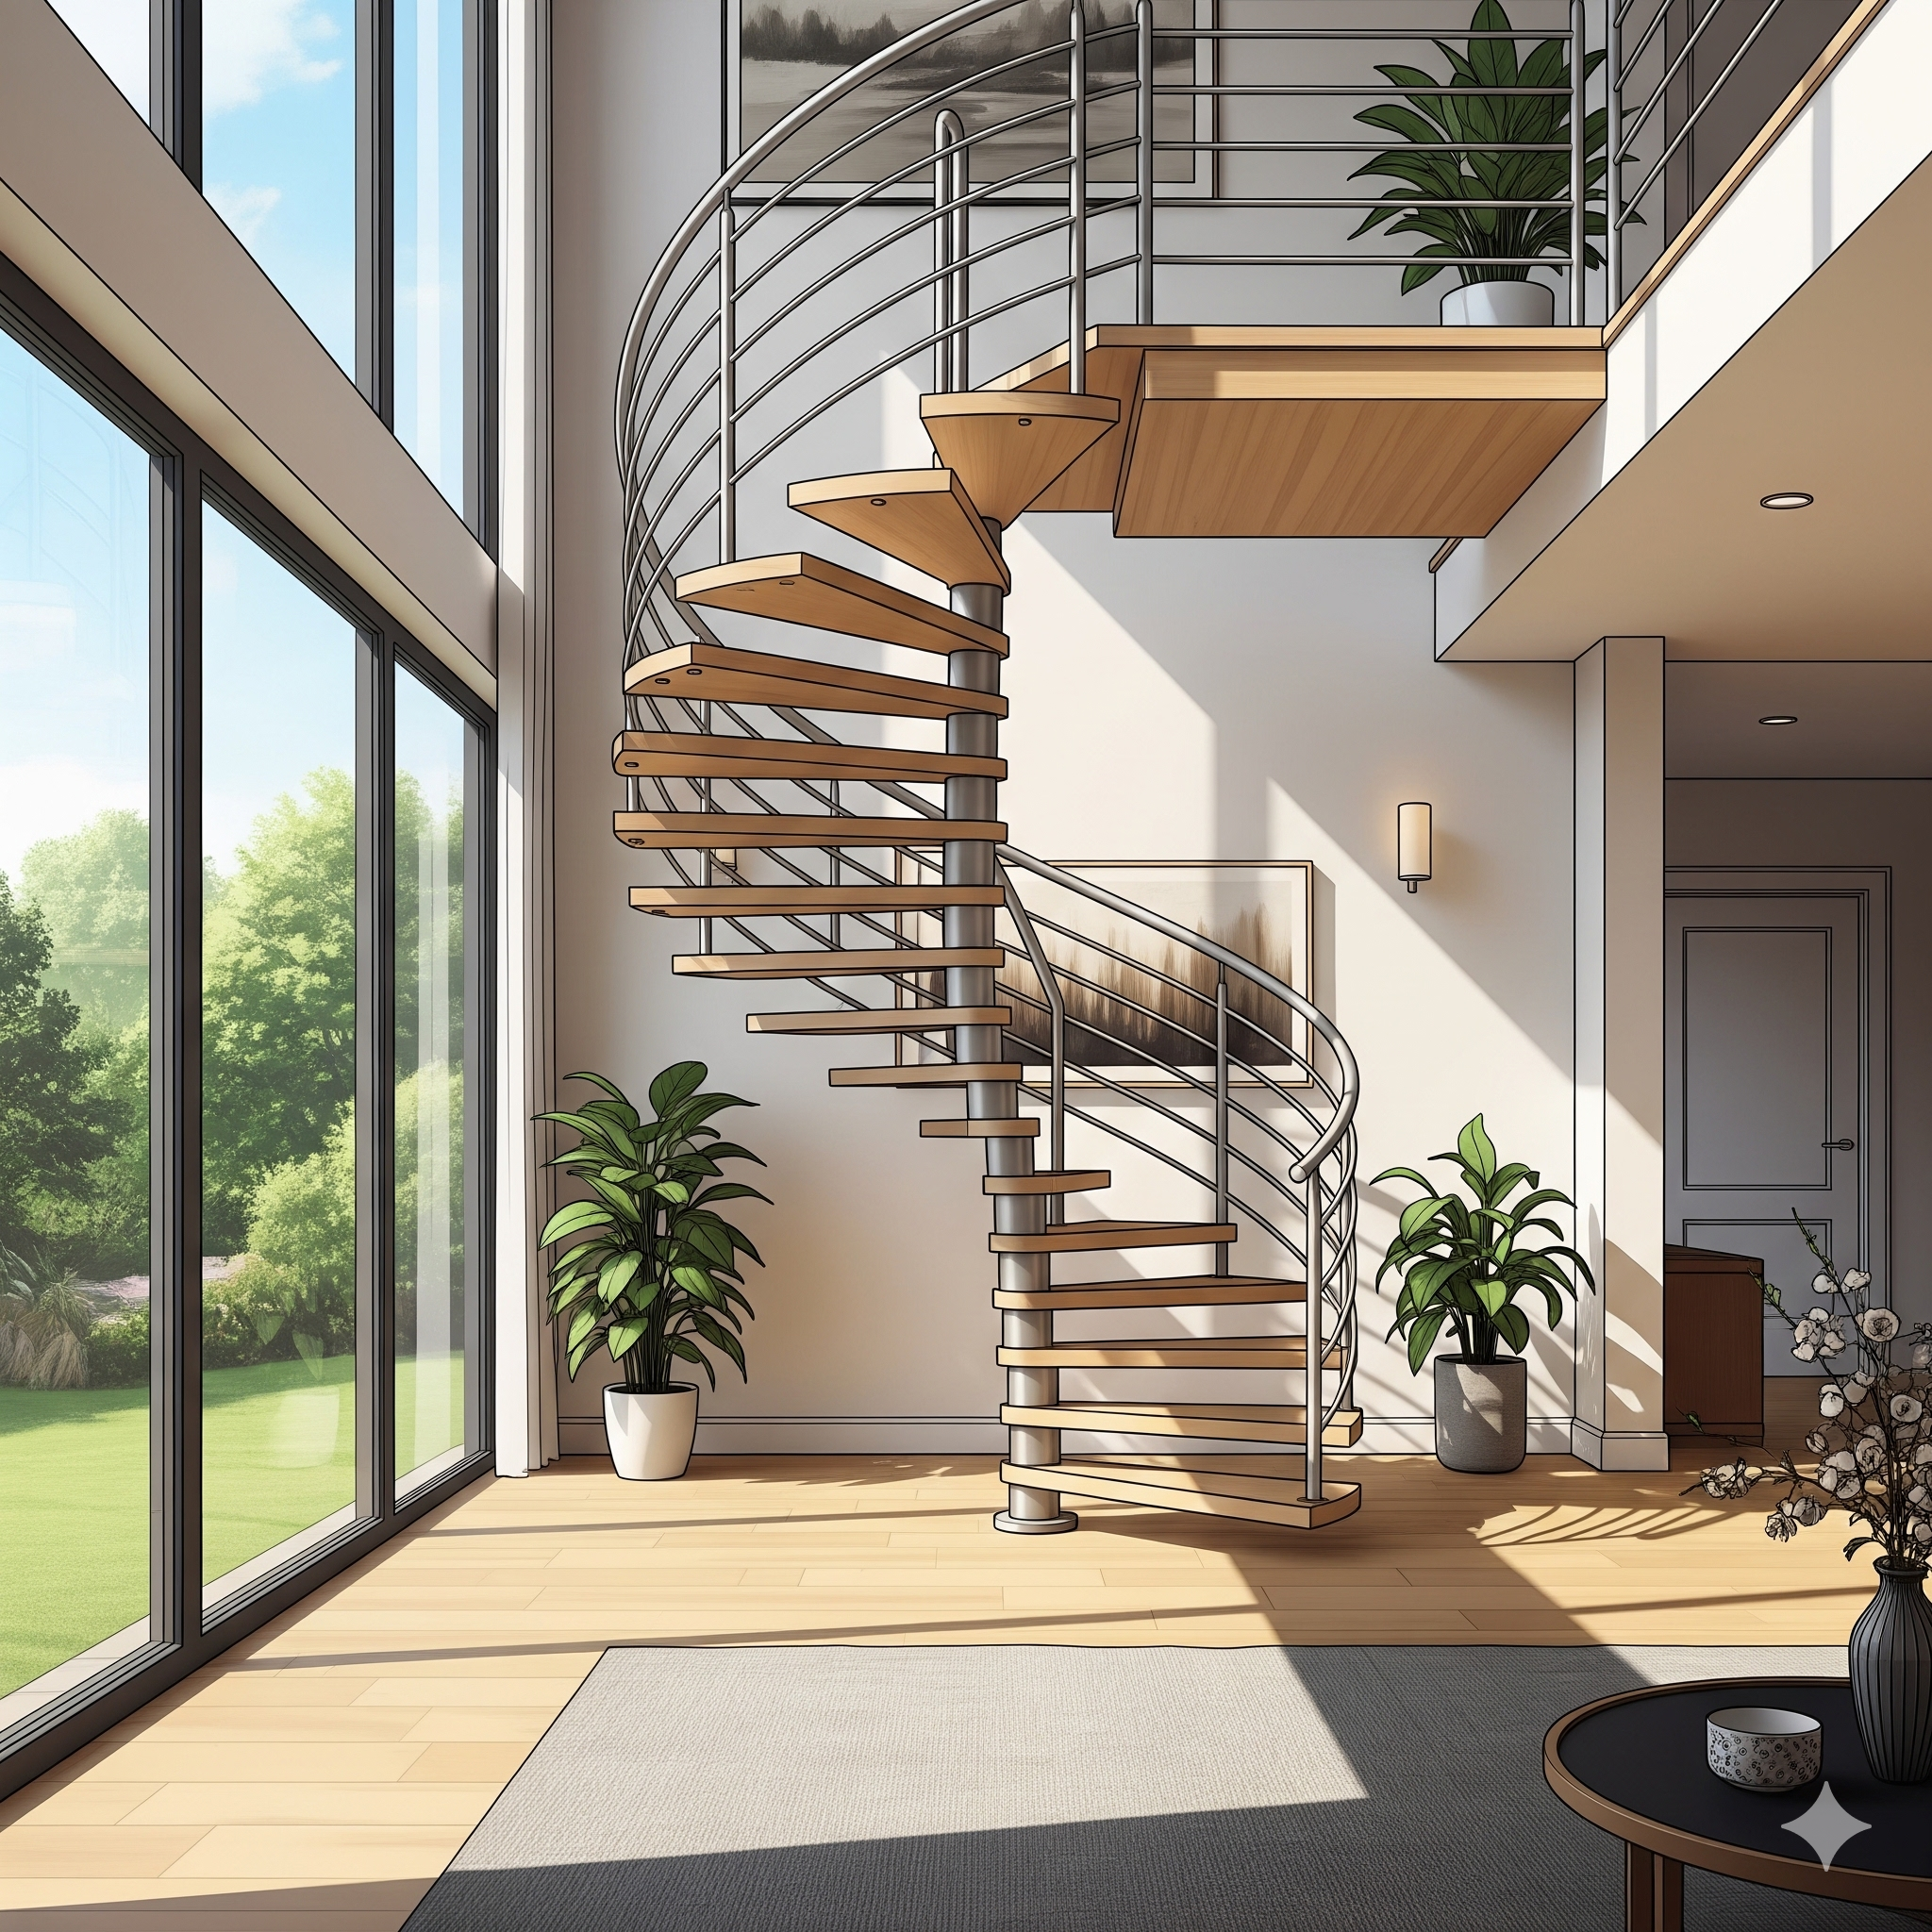
\includegraphics[width=0.4\linewidth]{figuras/9_ano/Escada.png}
        \end{figure}
        A professora Elielma sobe essa escada pisando na ponta de cada degrau para chegar ao seu quarto. Ao meio-dia, o sol está a pino e seus raios de luz incidem de forma perfeitamente perpendicular (formando um ângulo de 90°) em relação ao chão plano da sala. Qual figura geométrica plana o desenho da sombra gerada formaria?
        \begin{multicols}{4}
            \begin{enumerate}[label=\alph*)]
                \item Uma espiral
                \item um retângulo
                \item um círculo
                \item uma reta
            \end{enumerate}
        \end{multicols}

\begin{solucoes}{1}
    \solucao

Nesta imagem, ao olharmos de cima veremos uma figura interessante,
        \begin{figure}[H]
            \centering
            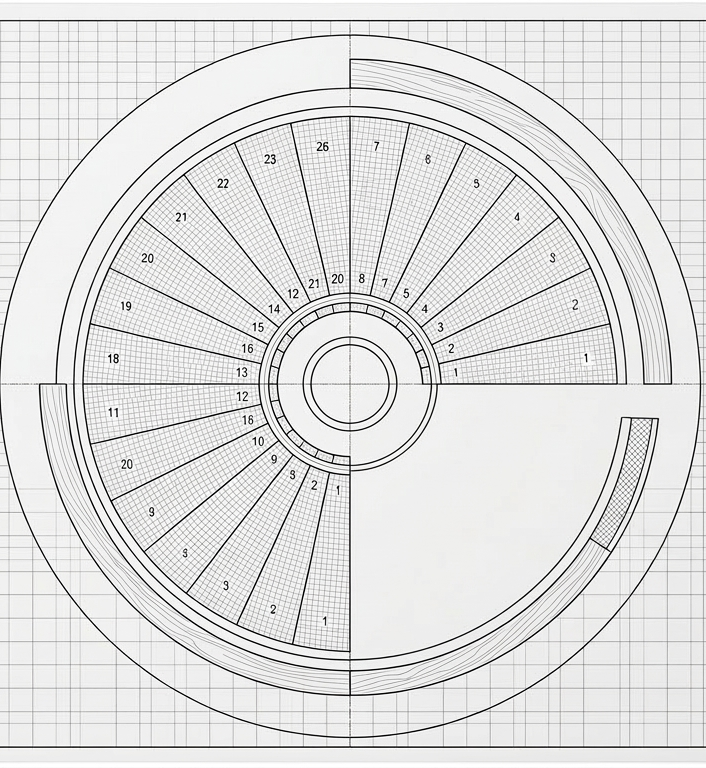
\includegraphics[width=0.4\linewidth]{figuras/9_ano/Projeção.png}
        \end{figure}
        Logo, a projeção ortogonal é dada por um círculo.\\
        \textbf{ALTERNATIVA C}
\end{solucoes}

\questao{(AUTORIA PRÓPRIA) Mostre que em um triângulo pitagórico, triângulo retângulo de lados inteiros, primitivo, o $mdc(x,y,z)=1$, os catetos possuem paridade diferente.}

\begin{solucoes}{1}
\solucao
Dizer que os catetos possuem paridade diferente é o mesmo que dizer que um deles deve ser par e o outro deve ser ímpar. Considere um triângulo pitagórico primitivo de lados $x,y$ e $z$, onde $x^2+y^2=z^2$ ($x$ e $y$ são os catetos e $z$ a hipotenusa) e $mdc(x,y,z)=1$. Para concluírmos o que se pede é preciso lembrar que só existem três possibilidades, ambos pares, ambos ímpares e terem paridade diferente. Mostremos por contradição que não podem ser ou ambos pares ou ambos ímpares,  

$i)$ Se ambos forem pares teríamos $x=2k$ e $y=2l$. Assim, 
\begin{equation*}
    x^2+y^2=(2k)^2+(2l)^2=4(k^2+l^2)=4p=z^2
\end{equation*}
O que é uma contradição, pois assim $z^2=$ é um múltiplo de 4 e $z$ é múltiplo de 2, o que não pode ocorrer,pois $mdc(x,y,z)=1$. Logo, $x$ e $y$ não podem ser ambos pares.

$ii)$ Se ambos forem ímpares teríamos $x=2k+1$ e $y=2l+1$ (Perceba que dizer que um número é ímpar é o mesmo que dizer que ele deixa resto $1$ quando dividido por $2$ ). Assim, 
\begin{equation*}
    x^2+y^2=(2k+1)^2+(2l+1)^2
\end{equation*}
\begin{equation*}
    x^2+y^2=4k^2+4k+1+4l^2+4l+1=4(k^2+k+l^2+l)+2=4t+2=2(2t+1)=2p
\end{equation*}
Logo, duas coisas saltam aos olhos. Em primeiro lugar, mostramos que a soma do quadrado de dois números ímpares deixa resto $2$ na divisão por quatro e em segundo lugar, mostramos que $z^2$ é par e consequentemente $z=2r$ (deixa resto $0$ na divisão por $2$). Todavia, a segunda informação gera uma contradição, pois $x^2+y^2$ deixa resto $2$ na divisão por 4 e $z^2=(2r)^2=4r^2$ e sendo assim, deixaria resto $0$ na divisão por $4$. Logo, ambos não podem ser ímpares.


Portanto, como ambos não podem ser nem pares e nem ímpares, os catetos de um triângulo pitagórico primitivo possuem paridadesdiferentes.
\end{solucoes}


        